\section{Исследовательский раздел \hfill}
\vspace{\baselineskip}


\subsection{Технические характеристики}

Технические характеристики устройства, на котором выполнялись замеры времени:

\begin{itemize}[label=---]
	\item операционная система Windows 10;
	\item память 8 ГБ;
	\item процессор Intel® Core™ i5-6260U @ 1.80 ГГц, 2 физических ядра, 4 логических ядра.
\end{itemize}

Замеры времени выполнения реализаций алгоритмов проводились на ноутбуке, включенном в сеть электропитания. Во время тестирования ноутбук был нагружен только встроенными приложениями окружения, а также непосредственно разработанным приложением.

\subsection{Демонстрация работы программы}

На рисунках \ref{fig:output1}-\ref{fig:output2} представлены примеры работы программы для линейной реализации алгоритма и для реализации с использованием вычислительного конвейера соответственно.
\clearpage

\begin{figure}[h!btp]
	\centering
	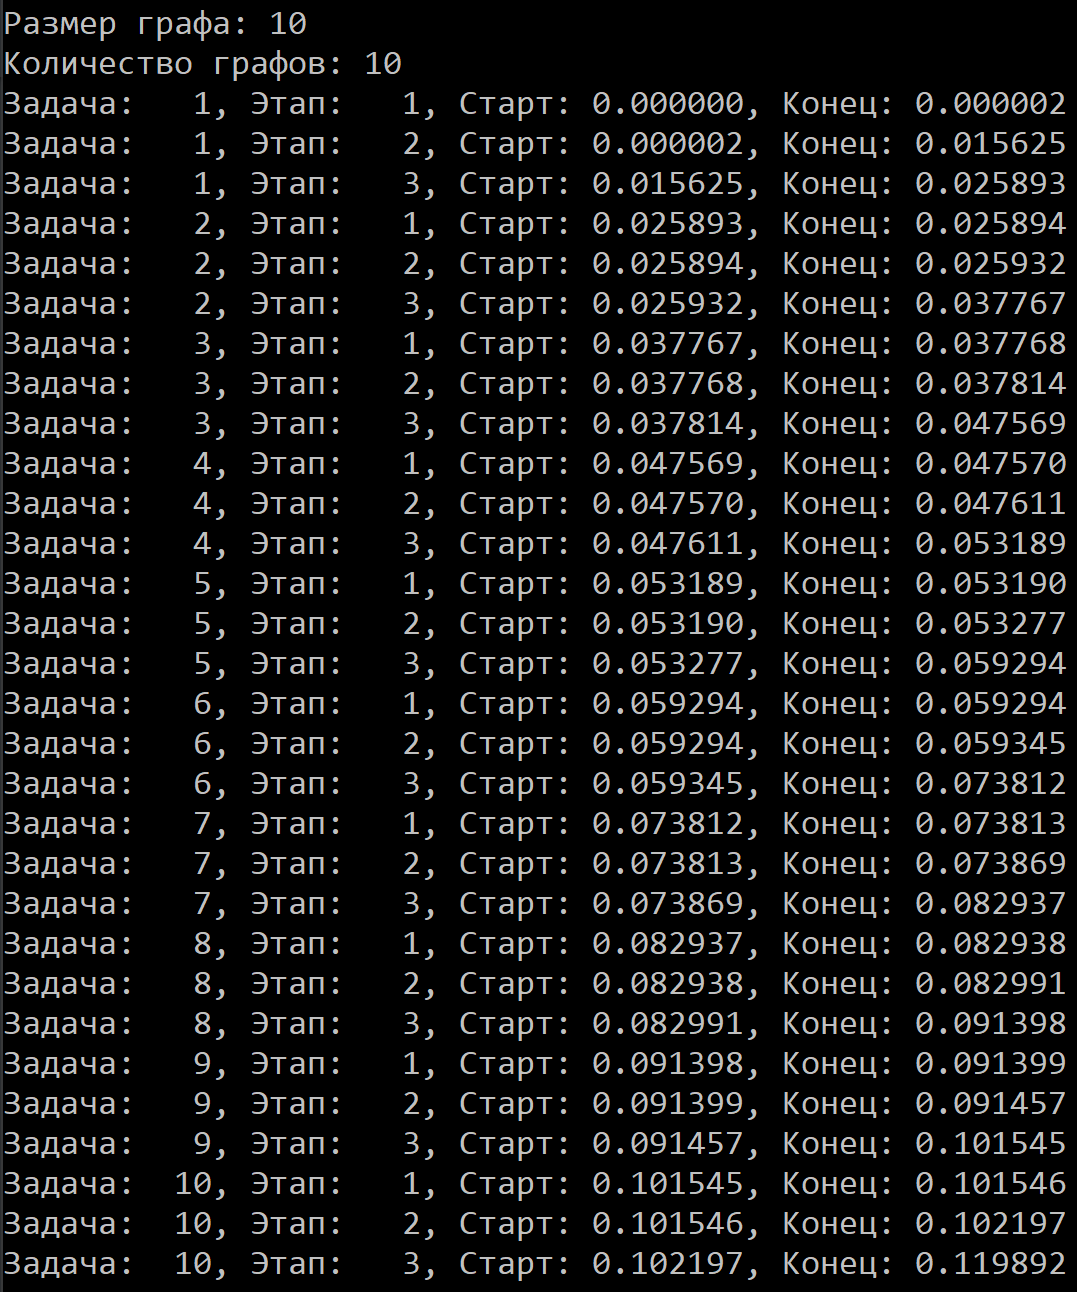
\includegraphics[width=240pt]{inc/output1.png}
	\caption{Пример работы линейной реализации алгоритма}
	\label{fig:output1}	
\end{figure}

\begin{figure}[h!btp]
	\centering
	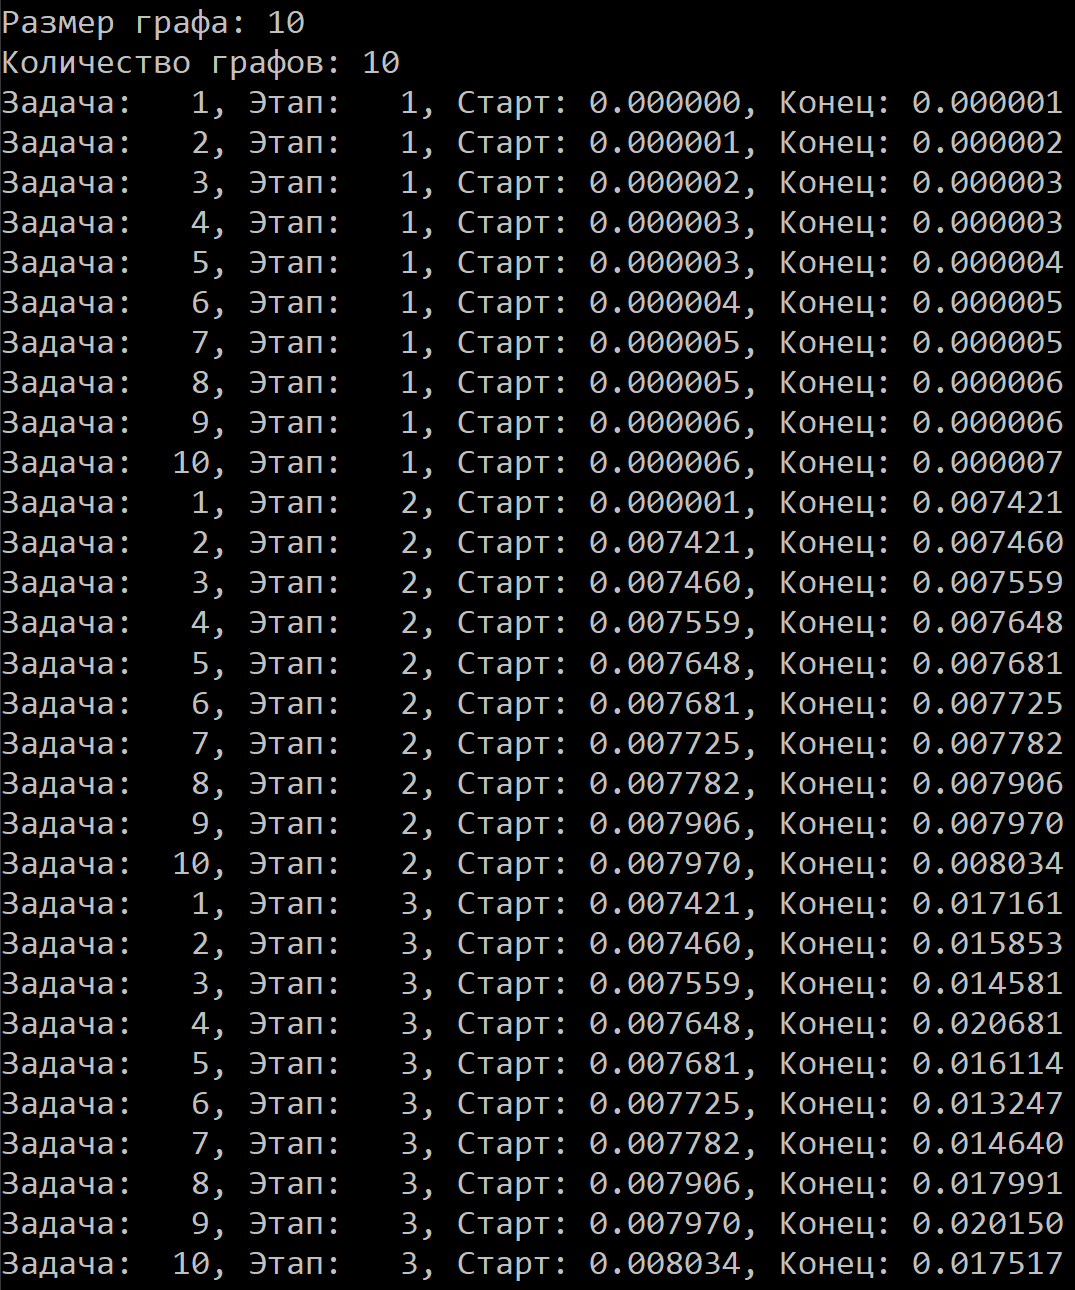
\includegraphics[width=240pt]{inc/output2.png}
	\caption{Пример работы реализации с использованием вычислительного конвейера}
	\label{fig:output2}	
\end{figure}

\subsection{Сравнение времени выполнения реализаций алгоритмов}

Сравнивается время работы последовательного алгоритма раскраски графа и раскраски графа с использованием параллельного конвейера на графах размером 5 и на количестве задач 1, 5, 25 и от 50 до 250 с шагом 50. Так как некоторые задачи выполняются достаточно быстро, а замеры времени имеют некоторую погрешность, они для каждой реализации и каждого количества задач выполняются 10 раз, а затем вычисляется среднее время работы.

В таблице \ref{tab:research} и на рисунке \ref{fig:research} приведены результаты сравнения времени выполнения реализаций алгоритмов.

\begin{table}[h]
    \begin{center}
    \begin{threeparttable}
        \captionsetup{justification=raggedright}
        \caption{\label{tab:research}Зависимость времени работы реализации от количества задач}
        \begin{tabular}{|p{0.2\linewidth}|p{0.35\linewidth}|p{0.35\linewidth}|}
            \hline
            \bfseries Количество задач & \bfseries Линейная \newline реализация (мс) & \bfseries Параллельная \newline реализация (мс) \\
            \hline
            1 & 0.015055 & 0.010745 \\
            \hline
            5 & 0.077368 & 0.011901 \\
            \hline
            25 & 0.243078 & 0.036809 \\
            \hline
            50 & 0.391589 & 0.093655 \\
            \hline
            100 & 0.830965 & 0.314735 \\
            \hline
            150 & 1.190327 & 0.414980 \\
            \hline
            200 & 1.550471 & 0.619565 \\
            \hline
            250 & 2.079744 & 0.856838 \\
            \hline
        \end{tabular}
    \end{threeparttable}
    \end{center}
\end{table} 
\clearpage

\begin{figure}[h!btp]
	\centering
	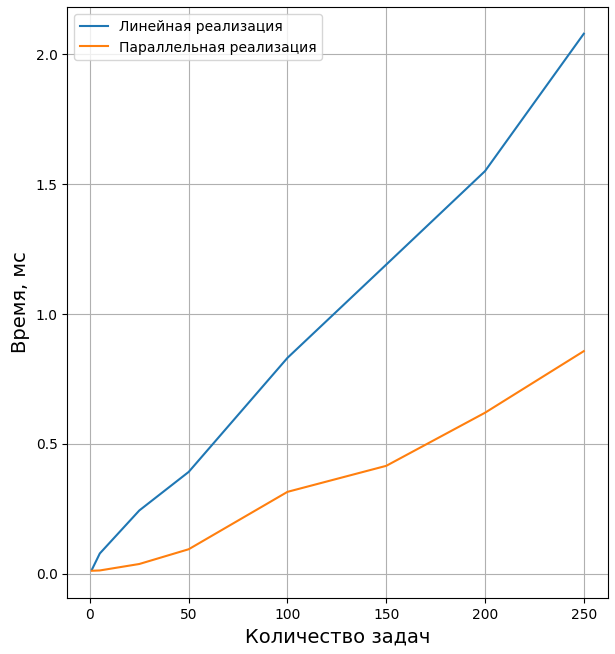
\includegraphics[width=300pt]{inc/research.png}
	\caption{Зависимость времени работы реализации от количества задач}
	\label{fig:research}	
\end{figure}

\subsection*{Вывод}
Реализация с использованием параллельного конвейера работает быстрее, чем линейная реализация.

Например, при количестве графов 100 параллельная реализация работает в 2.64 раза быстрее, чем линейная, а при количестве 250 -- в 2.43 раза. Уже при размере очереди в 5 элементов реализация вычислительного конвейера оправдывает себя.

Таким образом, конвейер позволяет существенно увеличить скорость выполнения задачи, разделив одну задачу на несколько простых.